% Options for packages loaded elsewhere
\PassOptionsToPackage{unicode}{hyperref}
\PassOptionsToPackage{hyphens}{url}
%
\documentclass[a4paper,11pt,twoside,pdftex,draft]{article}
\usepackage{lmodern}
\usepackage{amssymb,amsmath}
\usepackage{ifxetex,ifluatex}
\ifnum 0\ifxetex 1\fi\ifluatex 1\fi=0 % if pdftex
  \usepackage[T1]{fontenc}
  \usepackage[utf8]{inputenc}
  \usepackage{textcomp} % provide euro and other symbols
\else % if luatex or xetex
  \usepackage{unicode-math}
  \defaultfontfeatures{Scale=MatchLowercase}
  \defaultfontfeatures[\rmfamily]{Ligatures=TeX,Scale=1}
\fi
% Use upquote if available, for straight quotes in verbatim environments
\IfFileExists{upquote.sty}{\usepackage{upquote}}{}
\IfFileExists{microtype.sty}{% use microtype if available
  \usepackage[]{microtype}
  \UseMicrotypeSet[protrusion]{basicmath} % disable protrusion for tt fonts
}{}
\makeatletter
\@ifundefined{KOMAClassName}{% if non-KOMA class
  \IfFileExists{parskip.sty}{%
    \usepackage{parskip}
  }{% else
    \setlength{\parindent}{0pt}
    \setlength{\parskip}{6pt plus 2pt minus 1pt}}
}{% if KOMA class
  \KOMAoptions{parskip=half}}
\makeatother
\usepackage{xcolor}
\IfFileExists{xurl.sty}{\usepackage{xurl}}{} % add URL line breaks if available
\IfFileExists{bookmark.sty}{\usepackage{bookmark}}{\usepackage{hyperref}}
\hypersetup{
  hidelinks,
  pdfcreator={LaTeX via pandoc}}
\urlstyle{same} % disable monospaced font for URLs
\usepackage{longtable,booktabs}
% Correct order of tables after \paragraph or \subparagraph
\usepackage{etoolbox}
\makeatletter
\patchcmd\longtable{\par}{\if@noskipsec\mbox{}\fi\par}{}{}
\makeatother
% Allow footnotes in longtable head/foot
\IfFileExists{footnotehyper.sty}{\usepackage{footnotehyper}}{\usepackage{footnote}}
\makesavenoteenv{longtable}
\usepackage{graphicx}
\makeatletter
\def\maxwidth{\ifdim\Gin@nat@width>\linewidth\linewidth\else\Gin@nat@width\fi}
\def\maxheight{\ifdim\Gin@nat@height>\textheight\textheight\else\Gin@nat@height\fi}
\makeatother
% Scale images if necessary, so that they will not overflow the page
% margins by default, and it is still possible to overwrite the defaults
% using explicit options in \includegraphics[width, height, ...]{}
\setkeys{Gin}{width=\maxwidth,height=\maxheight,keepaspectratio}
% Set default figure placement to htbp
\makeatletter
\def\fps@figure{htbp}
\makeatother
\setlength{\emergencystretch}{3em} % prevent overfull lines
\providecommand{\tightlist}{%
  \setlength{\itemsep}{0pt}\setlength{\parskip}{0pt}}
\setcounter{secnumdepth}{-\maxdimen} % remove section numbering


% Geometry for A4 layout like MS-Word defaults
\usepackage[left=2.54cm,top=2.54cm,bottom=2.54cm,right=2.54cm]{geometry}


\date{}

\begin{document}

CASAL2

Software Architecture

v2016.1

Author:

\emph{Scott Rasmussen}

\emph{Zaita}

\emph{scott.rasmussen@zaita.com}

Table of Contents

\protect\hyperlink{document-history}{Document History 3}

\protect\hyperlink{casal2-overview}{iSAM Overview 3}

\protect\hyperlink{supported-operating-systems}{Supported Software
Requirements 3}

\protect\hyperlink{development-environment}{Development Environment 4}

\protect\hyperlink{operating-systems}{Operating Systems 4}

\protect\hyperlink{development-environment-1}{Development Environment 4}

\protect\hyperlink{windows}{Windows 4}

\protect\hyperlink{linux}{Linux 4}

\protect\hyperlink{both}{Both 4}

\protect\hyperlink{coding-style}{Coding Style 4}

\protect\hyperlink{high-level-design}{High-Level Design 5}

\protect\hyperlink{level-0-data-flow-diagram}{Level 0 Data-Flow-Diagram
5}

\protect\hyperlink{state-transition-diagram}{State-Transition Diagram 5}

\protect\hyperlink{state-descriptions}{State Descriptions 6}

\protect\hyperlink{startup}{StartUp 6}

\protect\hyperlink{validate}{Validate 6}

\protect\hyperlink{build}{Build 6}

\protect\hyperlink{verify}{Verify 6}

\protect\hyperlink{preexecute}{PreExecute 7}

\protect\hyperlink{execute}{Execute 7}

\protect\hyperlink{postexecute}{PostExecute 7}

\protect\hyperlink{iterationcomplete}{IterationComplete 7}

\protect\hyperlink{reset}{Reset 7}

\protect\hyperlink{finalise}{Finalise 7}

\protect\hyperlink{software-components}{Software Components 8}

\protect\hyperlink{utilities-library}{Utilities Library 8}

\protect\hyperlink{configuration-file-parser}{Configuration File Parser
8}

\protect\hyperlink{__RefHeading__689_571873561}{Equation Parser 8}

\protect\hyperlink{minimisers}{Minimisers 8}

\protect\hyperlink{__RefHeading__693_571873561}{State-Model 9}

\protect\hyperlink{plugin-architecture}{Plugin Architecture 9}

\protect\hyperlink{dynamic-library}{Dynamic-Library 9}

\protect\hyperlink{command-line-executable}{Command-Line Executable 9}

\protect\hyperlink{equation-parser}{Equation Parser 10}

\protect\hyperlink{__RefHeading__681_571873561}{OpenCL Kernel 10}

\protect\hyperlink{population-processes}{Population Processes 11}

\protect\hyperlink{category-shifting}{Category Shifting 11}

\protect\hyperlink{recruitment}{Recruitment 11}

\protect\hyperlink{mortality}{Mortality 11}

\protect\hyperlink{ageinggrowth}{Ageing/Growth 11}

\protect\hyperlink{software-integrity}{Software Integrity 12}

\hypertarget{document-history}{%
\section{Document History}\label{document-history}}

\begin{longtable}[]{@{}llll@{}}
\toprule
\endhead
Version & Description & Author & Date\tabularnewline
1.0 & \emph{Initial version - Draft} & S.Rasmussen &
13/06/2012\tabularnewline
1.1 & \emph{Modification of diagrams, explanation of states} &
S.Rasmussen & 12/07/2012\tabularnewline
1.2 & \emph{Updating diagram to show modifications to states} &
S.Rasmussen & 28/02/2013\tabularnewline
& \emph{Updating Development environment} & &\tabularnewline
1.3 & \emph{Update to show functionality created as part of phase 1} &
S.Rasmussen & 05/07/2013\tabularnewline
V2016.1 & \emph{Update to reflect released version 1.0 of CASAL2} &
S.Rasmussen & 20/01/2016\tabularnewline
\bottomrule
\end{longtable}

\hypertarget{casal2-overview}{%
\section{CASAL2 Overview}\label{casal2-overview}}

CASAL2 is the successor to the CASAL modelling application that was
developed approximately 10 years ago. It has been developed using modern
technology and current best practice development techniques to ensure
maintainability and integrity.

CASAL2's architect is based on the design mentality behind the Spatial
Population Model (SPM -
\href{http://www.niwa.co.nz/fisheries/tools-resources/spm-spatial-population-model}{{http://www.niwa.co.nz/fisheries/tools-resources/spm-spatial-population-model}}
). The code base is highly modular with code developed in small
light-weight objects that are easily recognisable and extensible.

The SPM code base was developed in 2007 and is still maintainable today
as the code follows a well documented coding standard and a simplistic
layout for objects. The techniques used to develop SPM are proven, and
have been applied to the development of CASAL2.

\hypertarget{supported-operating-systems}{%
\section{Supported Operating
Systems}\label{supported-operating-systems}}

CASAL2 is as a native 64 bit (x64) application with no 32 bit (x86)
support.

The processor families supported are the Intel and AMD processors that
conform to the AMD64 (x64) specification. PowerPC and ARM processors are
not supported.

Operating Systems supported will be Windows 7/8/10 (64 bit) and Linux
(64 bit). All other Operating System variants (BSD, Unix, OSX, Android,
IOS) may work, but have not been tested.

\hypertarget{development-environment}{%
\section{\texorpdfstring{\textbf{Development
Environment}}{Development Environment}}\label{development-environment}}

CASAL2 will primarily be developed on:

\hypertarget{operating-systems}{%
\subsection{Operating Systems}\label{operating-systems}}

\begin{itemize}
\item
  Microsoft Windows 7 (x64)
\item
  Microsoft Windows 10
\item
  OpenSuSe 12.2 (Mantis x64)
\item
  OpenSuSe Tumbleweed (bleeding edge rolling releases)
\item
  Ubuntu 15.10

  \begin{enumerate}
  \item ~
    \hypertarget{development-environment-1}{%
    \subsection{Development
    Environment}\label{development-environment-1}}
  \end{enumerate}
\end{itemize}

The environments listed below contain the compatable versions. Any
versions of software not listed below are most likely not compatable
with CASAL2.

The G++ compiler must be atleast version 4.8 to work. Anything newer
than this should work fine.

\hypertarget{windows}{%
\subsubsection{Windows}\label{windows}}

\begin{itemize}
\item
  TDM-GCC 4.8.X
  (\href{http://tdm-gcc.tdragon.net/}{{http://tdm-gcc.tdragon.net/}} )
\item
  TDM-GCC 4.9.X
  (\href{http://tdm-gcc.tdragon.net/}{{http://tdm-gcc.tdragon.net/}} )
\item
  TDM-GCC 5.0.X
  (\href{http://tdm-gcc.tdragon.net/}{{http://tdm-gcc.tdragon.net/}} )
\item
  TDM-GCC 5.1.X
  (\href{http://tdm-gcc.tdragon.net/}{{http://tdm-gcc.tdragon.net/}} )
\item
  TDM-GFortran
\item
  AQTime3 -- Performance profiling
\item
  Very Sleepy -- Performance profiling

  CASAL2 comes with components as part of it's build system. These are:
\item
  Unix Utils - *nix command line applications for Windows
\item
  Python 2.X
\item
  CMake 2.8.X

  \begin{enumerate}
  \item ~
    \hypertarget{linux}{%
    \subsubsection{Linux}\label{linux}}
  \end{enumerate}
\end{itemize}

\begin{itemize}
\item
  GCC/G++ 4.8.X
\item
  GCC/G++ 4.9.X
\item
  GCC/G++ 5.0.X
\item
  GCC/G++ 5.1.X
\item
  GCC/G++ Fortran
\item
  Valgrind
\item
  CMake 2.8.X+
\item
  Python 2.X (not 3.X or 4.X)
\item
  Python dateutil, datetime, re, distutils modules

  \begin{enumerate}
  \item ~
    \hypertarget{both}{%
    \subsubsection{Both}\label{both}}
  \end{enumerate}
\end{itemize}

\begin{itemize}
\item
  Eclipse (\href{http://www.eclipse.org/}{{http://www.eclipse.org/}} )

  \begin{enumerate}
  \item ~
    \hypertarget{coding-style}{%
    \subsection{Coding Style}\label{coding-style}}

    While it's going to be a step away from the style used for SPM,
    CASAL2 will use the Google Coding style
    (\href{http://google-styleguide.googlecode.com/svn/trunk/cppguide.xml}{{http://google-styleguide.googlecode.com/svn/trunk/cppguide.xml}}
    ). Google provides a handy script to parse source code and highlight
    errors that do not match their coding style.

    Spelling of variable names, classes etc will all be done using
    British English.

    \emph{Note: The only deviation from this style is the use of *.cpp
    instead of *.cc for filename extensions.}
  \end{enumerate}
\end{itemize}

\begin{enumerate}
\setcounter{enumi}{3}
\item ~
  \hypertarget{high-level-design}{%
  \section{\texorpdfstring{\textbf{High-Level
  Design}}{High-Level Design}}\label{high-level-design}}

  \begin{enumerate}
  \item ~
    \hypertarget{level-0-data-flow-diagram}{%
    \subsection{Level 0
    Data-Flow-Diagram}\label{level-0-data-flow-diagram}}
  \end{enumerate}
\end{enumerate}

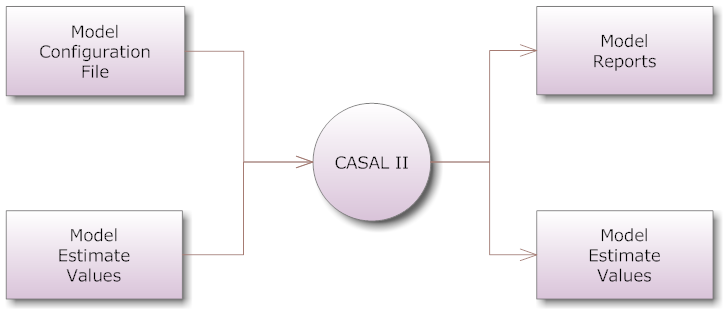
\includegraphics[width=6.0in,height=2.5in]{images/input_output.png}

\hypertarget{state-transition-diagram}{%
\subsection{State-Transition Diagram}\label{state-transition-diagram}}

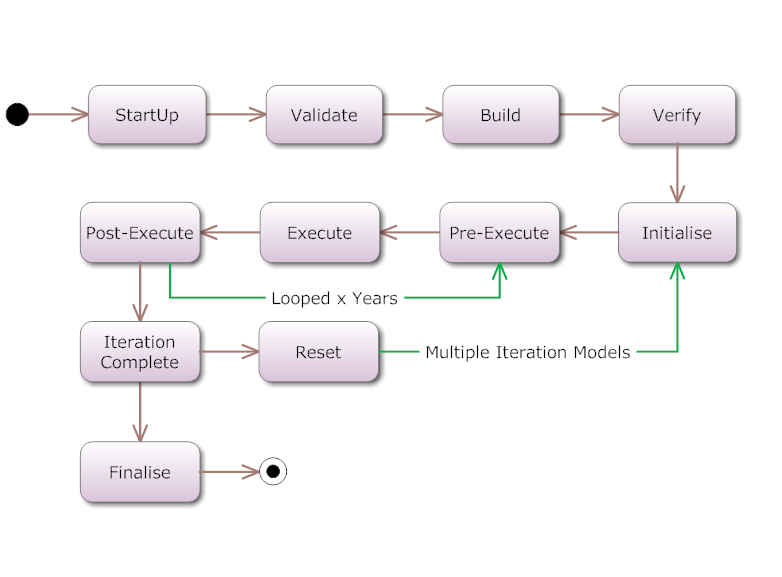
\includegraphics[width=6.0in,height=4.5in]{images/state_order.png}

\begin{enumerate}
\setcounter{enumi}{4}
\item ~
  \hypertarget{state-descriptions}{%
  \section{State Descriptions}\label{state-descriptions}}

  \begin{enumerate}
  \item ~
    \hypertarget{startup}{%
    \subsection{StartUp}\label{startup}}
  \end{enumerate}
\end{enumerate}

The model is in the blank start and the configuration system is loading
the configuration files and parsing any extra inputs.

Tasks completed:

\begin{itemize}
\item
  Parse command line
\item
  Parse configuration file
\item
  Load plugins
\item
  Load estimate values from input files

  \begin{enumerate}
  \item ~
    \hypertarget{validate}{%
    \subsection{Validate}\label{validate}}
  \end{enumerate}
\end{itemize}

All user configurations have been loaded at this point. Now the model
will go through every object that has been created and check that the
parameters given to them.

This step will ensure every object in the model has sufficient
parameters to be executed without causing a system fault or error in the
model.

This state will not check the values to ensure they are logical in
relation to an actual model. They will only test that they exist and
meet minimum requirements to execute a model.

At the end of the validate stage each object should be internally
consistent. No lookups or external references are allowed to be formed
during this stage.

\hypertarget{build}{%
\subsection{Build}\label{build}}

The build phase is where the system will build relationships between
objects that rely on each other. Because validation has been completed,
each object in it's self-contained configuration is ok.

This phase generally assigns values to pointers for objects so they
don't need to do lookups of objects during execution phases.

\hypertarget{verify}{%
\subsection{Verify}\label{verify}}

At this point pre-defined configurations are checked against the model's
current configuration to verify if the model makes sense logically.
These are business rules being applied to the model to help ensure the
output is not garbage.

\emph{Note: This state is not executed by default and must be defined as
part of the model execution.}

\textbf{Note: This has not been implemented.}

\hypertarget{preexecute}{%
\subsection{PreExecute}\label{preexecute}}

Pre-Execution happens at the beginning of a time step. This allows
objects to calculate values based on the partition state before any of
the other processes in the time step are executed.

\hypertarget{execute}{%
\subsection{Execute}\label{execute}}

This is the general work method of the model and where all of the
processes will be run against the partition.

\hypertarget{postexecute}{%
\subsection{PostExecute}\label{postexecute}}

This is executed at the end of a time step after all of the processes
and associated objects have been executed. This is typically used for
things like reports and derived quantities.

\hypertarget{iterationcomplete}{%
\subsection{IterationComplete}\label{iterationcomplete}}

This is executed at the end of every model run. This is only useful when
the model is in a multiple-iteration mode (e.g MCMC or Estimation).
After every model iteration this state is triggered.

\hypertarget{reset}{%
\subsection{Reset}\label{reset}}

If the model has to run multiple iterations then the reset state is used
to reset everything back in to a state where the model can be
re-executed without any legacy data remaining.

This state allows us to run multiple iterations of the model without
having to re-process the configuration information or
de-allocate/re-allocate large amounts of memory.

\hypertarget{finalise}{%
\subsection{Finalise}\label{finalise}}

Finalise will happen after all iterations of the model have been
completed.

\begin{enumerate}
\setcounter{enumi}{5}
\item ~
  \hypertarget{software-components}{%
  \section{Software Components}\label{software-components}}

  \begin{enumerate}
  \item ~
    \hypertarget{utilities-library}{%
    \subsection{Utilities Library}\label{utilities-library}}
  \end{enumerate}
\end{enumerate}

Inside CASAL2 is a collection of re-usable methods for reading the
command line, converting between types, using auto-differentiation
types, logging, error handling, double comparison etc.

While not a stand-alone library these methods can easily be extracted
for use within other NIWA projects.

\hypertarget{configuration-file-parser}{%
\subsection{Configuration File Parser}\label{configuration-file-parser}}

The configuration parser was developed from the ground up as a new
component for CASAL2 using ideas inspired by the SPM implementation.
While it's not a stand-alone component it is still in a state that
allows it to be easily ported to other applications.

Some of the in-built functionality of the configuration file parser is a
``parameters'' architecture that allows for quick retrieval and
validation of user supplied parameters with type-conversions and
validations. The configuration parser also has the ability to track what
file and line a particular parameter was defined to be used for error
reporting.

\emph{Note: it is expected that SPM will move to the same coding
standard as CASAL2 in the future and one of the first components that
will make a migration back from CASAL2 will be the configuration parsing
system.}

\hypertarget{minimisers}{%
\subsection{Minimisers}\label{minimisers}}

CASAL2 supports multiple minimisers out of the box.

\begin{itemize}
\item
  ADOL-C (Auto Differentiation)
\item
  BetaDiff (Auto-Differentiation)
\item
  CppAD (Auto-Differentiation)
\item
  GammaDiff / Numerical Differences
\item
  DESolver -- Differential Evolutionary Solver
\item
  DLib
\end{itemize}

Adding new minimisers is quite simple. Adding new minimisers that are
auto differentiation minimisers is significantly more complex, but still
a relatively simple task.

\hypertarget{section}{%
\section{\texorpdfstring{\hfill\break
}{ }}\label{section}}

\hypertarget{plugin-architecture}{%
\section{Plugin Architecture}\label{plugin-architecture}}

No plugin architecture has been developed. However adding the ability to
have objects loaded from shared libraries at runtime would be a simple
task. The main components of CASAL2 are already loaded like this, so
there is a heap of template code in the FrontEnd application.

\hypertarget{dynamic-library}{%
\subsection{Dynamic-Library}\label{dynamic-library}}

Developers with enough competence in C++ will be able to develop and
load their own plugins by building shared-libraries and specifying the
location of these within their configuration files.

An expected inclusion section of someone's plugin would be:

\#include \textless niwa/CASAL2/process.h\textgreater{}

\#include \textless niwa/CASAL2/selecvity.h\textgreater{}

class myNewProcess : public niwa::CASAL2::process \{

public:

void validate() \{ \}

void build() \{ \}

void execute() \{ \}

\}

\emph{Difficulty for user to develop:} High

\emph{Execution speed:} Fast

\hypertarget{command-line-executable}{%
\subsection{Command-Line Executable}\label{command-line-executable}}

Some components of the application will be replacable with command line
applications that take specific arguments and return a single result
(e.g Selectivities/Layers).

A specification will be developed to allow people to build and specify
stand-alone executable based plugins for specific functionality within
CASAL2 II.

The upside to this approach is that the user can specify any type of
executable they wish, developed in any language, including
shell-scripts. The application will simply do an exec() call on that
object and intepret the result.

\emph{Difficulty for user to develop:} Low

\emph{Execution speed:} Slow

\hypertarget{equation-parser}{%
\subsection{Equation Parser}\label{equation-parser}}

CASAL2 will have an inbuilt equation parser for handling equations
specified natively in the configuration file.

A valid example equation would be: 3\^{}x * 2

Where the user is able to bind 'x' to an internal parameter inside
CASAL2 II.

\emph{Difficulty for user to develop:} Low

\emph{Execution speed:} Slow

\hypertarget{section-1}{%
\section{\texorpdfstring{\hfill\break
}{ }}\label{section-1}}

\hypertarget{population-processes}{%
\section{Population Processes}\label{population-processes}}

CASAL2 supports a number of population processes. While there is a large
number of individual processes the general purpose of these can be
broken down in to a few different types.

Category shifting, recruitment, mortality and ageing/growth.

\hypertarget{category-shifting}{%
\subsection{Category Shifting}\label{category-shifting}}

These processes are responsible for moving part of the population from 1
category in to another.

Implemented in CASAL2 there is:

\begin{itemize}
\item
  Rate

  \begin{enumerate}
  \item ~
    \hypertarget{recruitment}{%
    \subsection{Recruitment}\label{recruitment}}
  \end{enumerate}
\end{itemize}

These processes are responsible for the introduction of new population
members.

Implemented in CASAL2 there is:

\begin{itemize}
\item
  Constant rate
\item
  Beverton-Holt

  \begin{enumerate}
  \item ~
    \hypertarget{mortality}{%
    \subsection{Mortality}\label{mortality}}
  \end{enumerate}
\end{itemize}

These processes are responsible for the removal of population members.

Implemented in CASAL2 there is:

\begin{itemize}
\item
  Constant rate
\item
  Event

  \begin{enumerate}
  \item ~
    \hypertarget{ageinggrowth}{%
    \subsection{Ageing/Growth}\label{ageinggrowth}}
  \end{enumerate}
\end{itemize}

These processes are responsible for moving population members up through
ages/lengths. They work similar to category shifting except only work
within a single category.

Implemented in CASAL2 there is:

\begin{itemize}
\item
  Ageing
\end{itemize}

\hypertarget{software-integrity}{%
\section{Software Integrity}\label{software-integrity}}

One of the key focusses in the CASAL2 development is the emphasis on
software integrity. It's hugely important to ensure results coming from
user models are consistent and correct.

As part of this we utilise unit tests to check individual components of
the software and run entire models verifying results.

CASAL2 uses:

\begin{itemize}
\item
  Google testing framework
\item
  Google mocking framework
\end{itemize}

As at 5\textsuperscript{th} July 2013 the unit test output was:

{[}=========={]} Running 19 tests from 4 test cases.

{[}-\/-\/-\/-\/-\/-\/-\/-\/-\/-{]} Global test environment set-up.

{[}-\/-\/-\/-\/-\/-\/-\/-\/-\/-{]} 7 tests from BasicModel

{[} RUN {]} BasicModel.Observation\_Abundance

{[} OK {]} BasicModel.Observation\_Abundance (3 ms)

{[} RUN {]} BasicModel.Accessors\_Cached\_CombinedCategories

{[} OK {]} BasicModel.Accessors\_Cached\_CombinedCategories (1 ms)

{[} RUN {]} BasicModel.Processes\_Constant\_Recruitment

{[} OK {]} BasicModel.Processes\_Constant\_Recruitment (1 ms)

{[} RUN {]} BasicModel.Processes\_Mortality\_Event\_No\_Penalty

{[} OK {]} BasicModel.Processes\_Mortality\_Event\_No\_Penalty (1 ms)

{[} RUN {]} BasicModel.Processes\_Mortality\_Constant\_Rate

{[} OK {]} BasicModel.Processes\_Mortality\_Constant\_Rate (1 ms)

{[} RUN {]}
BasicModel.Processes\_Maturation\_Rate\_Constant\_One\_Selectivity

{[} OK {]}
BasicModel.Processes\_Maturation\_Rate\_Constant\_One\_Selectivity (1
ms)

{[} RUN {]} BasicModel.Processes\_Ageing

{[} OK {]} BasicModel.Processes\_Ageing (1 ms)

{[}-\/-\/-\/-\/-\/-\/-\/-\/-\/-{]} 7 tests from BasicModel (10 ms total)

{[}-\/-\/-\/-\/-\/-\/-\/-\/-\/-{]} 1 test from PartitionAccessors

{[} RUN {]} PartitionAccessors.Category

{[} OK {]} PartitionAccessors.Category (0 ms)

{[}-\/-\/-\/-\/-\/-\/-\/-\/-\/-{]} 1 test from PartitionAccessors (0 ms
total)

{[}-\/-\/-\/-\/-\/-\/-\/-\/-\/-{]} 10 tests from Selectivities

{[} RUN {]} Selectivities.LogisticProducing

{[} OK {]} Selectivities.LogisticProducing (0 ms)

{[} RUN {]} Selectivities.Logistic

{[} OK {]} Selectivities.Logistic (0 ms)

{[} RUN {]} Selectivities.KnifeEdge

{[} OK {]} Selectivities.KnifeEdge (0 ms)

{[} RUN {]} Selectivities.InverseLogistic

{[} OK {]} Selectivities.InverseLogistic (0 ms)

{[} RUN {]} Selectivities.Increasing

{[} OK {]} Selectivities.Increasing (0 ms)

{[} RUN {]} Selectivities.DoubleNormal

{[} OK {]} Selectivities.DoubleNormal (0 ms)

{[} RUN {]} Selectivities.DoubleExponential

{[} OK {]} Selectivities.DoubleExponential (1 ms)

{[} RUN {]} Selectivities.Constant

{[} OK {]} Selectivities.Constant (0 ms)

{[} RUN {]} Selectivities.AllValuesBounded

{[} OK {]} Selectivities.AllValuesBounded (0 ms)

{[} RUN {]} Selectivities.AllValues

{[} OK {]} Selectivities.AllValues (0 ms)

{[}-\/-\/-\/-\/-\/-\/-\/-\/-\/-{]} 10 tests from Selectivities (2 ms
total)

{[}-\/-\/-\/-\/-\/-\/-\/-\/-\/-{]} Global test environment tear-down

{[}=========={]} 18 tests from 4 test cases ran. (14 ms total)

{[} PASSED {]} 18 tests.

A basic coverage of the currently implemented processes and
selectivities has already been achieved.

As of 20\textsuperscript{th} January 2016 the unit test output is:

Loading unit test DLL

{[}=========={]} Running 144 tests from 12 test cases.

{[}-\/-\/-\/-\/-\/-\/-\/-\/-\/-{]} Global test environment set-up.

{[}-\/-\/-\/-\/-\/-\/-\/-\/-\/-{]} 1 test from AdditionalPriors

{[} RUN {]} AdditionalPriors.Beta

{[} OK {]} AdditionalPriors.Beta (0 ms)

{[}-\/-\/-\/-\/-\/-\/-\/-\/-\/-{]} 1 test from AdditionalPriors (0 ms
total)

{[}-\/-\/-\/-\/-\/-\/-\/-\/-\/-{]} 72 tests from InternalEmptyModel

{[} RUN {]} InternalEmptyModel.AgeLengths\_Data\_Mean\_Mean

{[} OK {]} InternalEmptyModel.AgeLengths\_Data\_Mean\_Mean (314 ms)

{[} RUN {]} InternalEmptyModel.AgeLengths\_Data\_NearestNeighbour\_Mean

{[} OK {]} InternalEmptyModel.AgeLengths\_Data\_NearestNeighbour\_Mean
(305 ms)

{[} RUN {]} InternalEmptyModel.AgeLengths\_Data\_Mean\_NearestNeighbour

{[} OK {]} InternalEmptyModel.AgeLengths\_Data\_Mean\_NearestNeighbour
(306 ms)

{[} RUN {]} InternalEmptyModel.AgeLengths\_Data\_Mean\_Interpolate

{[} OK {]} InternalEmptyModel.AgeLengths\_Data\_Mean\_Interpolate (312
ms)

{[} RUN {]} InternalEmptyModel.Asserts\_Estimable

{[} OK {]} InternalEmptyModel.Asserts\_Estimable (6 ms)

{[} RUN {]} InternalEmptyModel.Asserts\_Estimable\_Throws\_Exception

{[}ERROR{]}
/home/zaita/CASAL2/CASAL2/source/Asserts/Children/Estimable.cpp(line:
88): Assert Failure: Estimable: process{[}Recruitment{]}.R0 had actual
value 997386 when we expected 1

{[} OK {]} InternalEmptyModel.Asserts\_Estimable\_Throws\_Exception (5
ms)

{[} RUN {]} InternalEmptyModel.Asserts\_ObjectiveFunction

{[} OK {]} InternalEmptyModel.Asserts\_ObjectiveFunction (6 ms)

{[} RUN {]}
InternalEmptyModel.Asserts\_ObjectiveFunction\_Throws\_Exception

{[}ERROR{]}
/home/zaita/CASAL2/CASAL2/source/Asserts/Children/ObjectiveFunction.cpp(line:
49): Assert Failure: Objective Function had actual value 13.8129 when we
expected 1 with difference: 12

{[} OK {]}
InternalEmptyModel.Asserts\_ObjectiveFunction\_Throws\_Exception (5 ms)

{[} RUN {]}
InternalEmptyModel.Categories\_AssignSpecificYearsPerCategory\_1

{[} OK {]}
InternalEmptyModel.Categories\_AssignSpecificYearsPerCategory\_1 (1 ms)

{[} RUN {]}
InternalEmptyModel.Categories\_AssignSpecificYearsPerCategory\_2

{[}ERROR{]}
/home/zaita/CASAL2/CASAL2/source/Categories/Categories.cpp(line: 128):
At line 98 in
/home/zaita/CASAL2/CASAL2/source/Categories/Categories.Test.cpp the
parameter 'years' value 2000 has already been defined for the category
male.immature.2000

{[} OK {]}
InternalEmptyModel.Categories\_AssignSpecificYearsPerCategory\_2 (0 ms)

{[} RUN {]}
InternalEmptyModel.Categories\_AssignSpecificYearsPerCategory\_3

{[} OK {]}
InternalEmptyModel.Categories\_AssignSpecificYearsPerCategory\_3 (1 ms)

{[} RUN {]}
InternalEmptyModel.Categories\_AssignSpecificYearsPerCategory\_4

{[} OK {]}
InternalEmptyModel.Categories\_AssignSpecificYearsPerCategory\_4 (0 ms)

{[} RUN {]}
InternalEmptyModel.Categories\_AssignSpecificYearsPerCategory

{[} OK {]} InternalEmptyModel.Categories\_AssignSpecificYearsPerCategory
(0 ms)

{[} RUN {]} InternalEmptyModel.Categories\_GetCategoryLabels

{[} OK {]} InternalEmptyModel.Categories\_GetCategoryLabels (1 ms)

{[} RUN {]} InternalEmptyModel.DerivedQuantities\_Abundance

{[} OK {]} InternalEmptyModel.DerivedQuantities\_Abundance (1 ms)

{[} RUN {]} InternalEmptyModel.DerivedQuantities\_Biomass

{[} OK {]} InternalEmptyModel.DerivedQuantities\_Biomass (0 ms)

{[} RUN {]} InternalEmptyModel.EstimateTransformations\_Inverse

{[} OK {]} InternalEmptyModel.EstimateTransformations\_Inverse (558 ms)

{[} RUN {]}
InternalEmptyModel.EstimateTransformations\_Inverse\_NoBounds

{[} OK {]} InternalEmptyModel.EstimateTransformations\_Inverse\_NoBounds
(499 ms)

{[} RUN {]}
InternalEmptyModel.EstimateTransformations\_Inverse\_NoBounds\_With\_DLib\_Minimiser

{[} OK {]}
InternalEmptyModel.EstimateTransformations\_Inverse\_NoBounds\_With\_DLib\_Minimiser
(6901 ms)

{[} RUN {]}
InternalEmptyModel.EstimateTransformations\_Inverse\_NoBounds\_With\_DeSolver\_Minimiser

{[} OK {]}
InternalEmptyModel.EstimateTransformations\_Inverse\_NoBounds\_With\_DeSolver\_Minimiser
(1301 ms)

{[} RUN {]} InternalEmptyModel.EstimateTransformations\_Log

{[} OK {]} InternalEmptyModel.EstimateTransformations\_Log (509 ms)

{[} RUN {]} InternalEmptyModel.EstimateTransformations\_Log\_NoBounds

{[} OK {]} InternalEmptyModel.EstimateTransformations\_Log\_NoBounds
(990 ms)

{[} RUN {]}
InternalEmptyModel.EstimateTransformations\_Log\_With\_DLib\_Minimiser

{[} OK {]}
InternalEmptyModel.EstimateTransformations\_Log\_With\_DLib\_Minimiser
(6970 ms)

{[} RUN {]}
InternalEmptyModel.EstimateTransformations\_Log\_With\_DeSolver\_Minimiser

{[} OK {]}
InternalEmptyModel.EstimateTransformations\_Log\_With\_DeSolver\_Minimiser
(1306 ms)

{[} RUN {]} InternalEmptyModel.EstimateTransformations\_SquareRoot

{[} OK {]} InternalEmptyModel.EstimateTransformations\_SquareRoot (697
ms)

{[} RUN {]}
InternalEmptyModel.EstimateTransformations\_SquareRoot\_NoBounds

{[} OK {]}
InternalEmptyModel.EstimateTransformations\_SquareRoot\_NoBounds (1205
ms)

{[} RUN {]}
InternalEmptyModel.EstimateTransformations\_SquareRoot\_With\_DLib\_Minimiser

{[} OK {]}
InternalEmptyModel.EstimateTransformations\_SquareRoot\_With\_DLib\_Minimiser
(3607 ms)

{[} RUN {]}
InternalEmptyModel.EstimateTransformations\_SquareRoot\_With\_DeSolver\_Minimiser

{[} OK {]}
InternalEmptyModel.EstimateTransformations\_SquareRoot\_With\_DeSolver\_Minimiser
(1301 ms)

{[} RUN {]} InternalEmptyModel.Estimates\_Beta

{[} OK {]} InternalEmptyModel.Estimates\_Beta (79 ms)

{[} RUN {]} InternalEmptyModel.Estimates\_Lognormal

{[} OK {]} InternalEmptyModel.Estimates\_Lognormal (74 ms)

{[} RUN {]} InternalEmptyModel.Estimates\_Normal

{[} OK {]} InternalEmptyModel.Estimates\_Normal (75 ms)

{[} RUN {]} InternalEmptyModel.Estimates\_Normal\_By\_Stdev

{[} OK {]} InternalEmptyModel.Estimates\_Normal\_By\_Stdev (75 ms)

{[} RUN {]} InternalEmptyModel.Estimates\_Normal\_Log

{[} OK {]} InternalEmptyModel.Estimates\_Normal\_Log (75 ms)

{[} RUN {]} InternalEmptyModel.Estimates\_Uniform

{[} OK {]} InternalEmptyModel.Estimates\_Uniform (76 ms)

{[} RUN {]} InternalEmptyModel.Estimates\_Uniform\_Log

{[} OK {]} InternalEmptyModel.Estimates\_Uniform\_Log (74 ms)

{[} RUN {]} InternalEmptyModel.Estimates\_Single\_Target

{[} OK {]} InternalEmptyModel.Estimates\_Single\_Target (81 ms)

{[} RUN {]}
InternalEmptyModel.Estimates\_Multiple\_Defined\_Targets\_Vector

{[} OK {]}
InternalEmptyModel.Estimates\_Multiple\_Defined\_Targets\_Vector (2472
ms)

{[} RUN {]}
InternalEmptyModel.Estimates\_Multiple\_Defined\_Targets\_Unsigned\_Map

{[} OK {]}
InternalEmptyModel.Estimates\_Multiple\_Defined\_Targets\_Unsigned\_Map
(39 ms)

{[} RUN {]}
InternalEmptyModel.Estimates\_Multiple\_Defined\_Targets\_String\_Map

{[} OK {]}
InternalEmptyModel.Estimates\_Multiple\_Defined\_Targets\_String\_Map
(33 ms)

{[} RUN {]} InternalEmptyModel.Estimates\_All\_Targets\_Vector

{[} OK {]} InternalEmptyModel.Estimates\_All\_Targets\_Vector (367 ms)

{[} RUN {]} InternalEmptyModel.Estimates\_All\_Targets\_Unsigned\_Map

{[} OK {]} InternalEmptyModel.Estimates\_All\_Targets\_Unsigned\_Map (75
ms)

{[} RUN {]} InternalEmptyModel.Estimates\_All\_Targets\_String\_Map

{[} OK {]} InternalEmptyModel.Estimates\_All\_Targets\_String\_Map (34
ms)

{[} RUN {]} InternalEmptyModel.Observation\_Process\_Abundance

{[} OK {]} InternalEmptyModel.Observation\_Process\_Abundance (6 ms)

{[} RUN {]} InternalEmptyModel.Observation\_Process\_Biomass

{[} OK {]} InternalEmptyModel.Observation\_Process\_Biomass (6 ms)

{[} RUN {]}
InternalEmptyModel.Observation\_Process\_Proportions\_At\_Age\_Single

{[} OK {]}
InternalEmptyModel.Observation\_Process\_Proportions\_At\_Age\_Single (6
ms)

{[} RUN {]}
InternalEmptyModel.Observation\_Process\_Proportions\_At\_Age\_Double

{[} OK {]}
InternalEmptyModel.Observation\_Process\_Proportions\_At\_Age\_Double (6
ms)

{[} RUN {]}
InternalEmptyModel.Observation\_Process\_Proportions\_At\_Age\_for\_fishery\_Single

{[} OK {]}
InternalEmptyModel.Observation\_Process\_Proportions\_At\_Age\_for\_fishery\_Single
(11 ms)

{[} RUN {]}
InternalEmptyModel.Observation\_Proportions\_At\_Length\_for\_fishery\_Single

{[} OK {]}
InternalEmptyModel.Observation\_Proportions\_At\_Length\_for\_fishery\_Single
(3 ms)

{[} RUN {]} InternalEmptyModel.Observation\_Biomass

{[} OK {]} InternalEmptyModel.Observation\_Biomass (6 ms)

{[} RUN {]} InternalEmptyModel.Observation\_Proportions\_At\_Age\_Single

{[} OK {]} InternalEmptyModel.Observation\_Proportions\_At\_Age\_Single
(5 ms)

{[} RUN {]} InternalEmptyModel.Observation\_Proportions\_At\_Age\_Double

{[} OK {]} InternalEmptyModel.Observation\_Proportions\_At\_Age\_Double
(6 ms)

{[} RUN {]}
InternalEmptyModel.Observation\_Proportions\_At\_Length\_Single

{[} OK {]}
InternalEmptyModel.Observation\_Proportions\_At\_Length\_Single (3 ms)

{[} RUN {]}
InternalEmptyModel.Observation\_Proportions\_At\_Length\_Double

{[} OK {]}
InternalEmptyModel.Observation\_Proportions\_At\_Length\_Double (0 ms)

{[} RUN {]}
InternalEmptyModel.Processes\_Mortality\_Instantaneous\_Simple

{[} OK {]}
InternalEmptyModel.Processes\_Mortality\_Instantaneous\_Simple (8 ms)

{[} RUN {]} InternalEmptyModel.Processes\_BevertonHolt\_Recruitment

{[} OK {]} InternalEmptyModel.Processes\_BevertonHolt\_Recruitment (11
ms)

{[} RUN {]}
InternalEmptyModel.Processes\_BevertonHolt\_Recruitment\_AutoSSBOffset

{[} OK {]}
InternalEmptyModel.Processes\_BevertonHolt\_Recruitment\_AutoSSBOffset
(1 ms)

{[} RUN {]} InternalEmptyModel.Processes\_Tag\_By\_Age

{[} OK {]} InternalEmptyModel.Processes\_Tag\_By\_Age (1 ms)

{[} RUN {]} InternalEmptyModel.Processes\_Tag\_By\_Age\_With\_Loss\_Rate

{[} OK {]} InternalEmptyModel.Processes\_Tag\_By\_Age\_With\_Loss\_Rate
(1 ms)

{[} RUN {]}
InternalEmptyModel.Processes\_Tag\_By\_Age\_With\_Loss\_Rate\_Selectivities

{[} OK {]}
InternalEmptyModel.Processes\_Tag\_By\_Age\_With\_Loss\_Rate\_Selectivities
(1 ms)

{[} RUN {]}
InternalEmptyModel.Processes\_Tag\_By\_Age\_With\_Selectivities

{[} OK {]}
InternalEmptyModel.Processes\_Tag\_By\_Age\_With\_Selectivities (1 ms)

{[} RUN {]}
InternalEmptyModel.Processes\_Tag\_By\_Age\_With\_Proportions\_Table

{[} OK {]}
InternalEmptyModel.Processes\_Tag\_By\_Age\_With\_Proportions\_Table (1
ms)

{[} RUN {]} InternalEmptyModel.Processes\_Transition\_Category\_By\_Age

{[} OK {]} InternalEmptyModel.Processes\_Transition\_Category\_By\_Age
(3 ms)

{[} RUN {]} InternalEmptyModel.Model\_CasalComplex1\_BasicRun

{[} OK {]} InternalEmptyModel.Model\_CasalComplex1\_BasicRun (11 ms)

{[} RUN {]} InternalEmptyModel.Model\_CasalComplex1\_Estimation

{[} OK {]} InternalEmptyModel.Model\_CasalComplex1\_Estimation (2556 ms)

{[} RUN {]} InternalEmptyModel.Model\_CasalComplex1\_Simulation

{[} OK {]} InternalEmptyModel.Model\_CasalComplex1\_Simulation (11 ms)

{[} RUN {]} InternalEmptyModel.Model\_CasalComplex2\_BasicRun

{[} OK {]} InternalEmptyModel.Model\_CasalComplex2\_BasicRun (14 ms)

{[} RUN {]} InternalEmptyModel.Model\_CasalComplex2\_Estimation

{[} OK {]} InternalEmptyModel.Model\_CasalComplex2\_Estimation (12106
ms)

{[} RUN {]} InternalEmptyModel.Model\_CasalComplex3\_BasicRun

{[} OK {]} InternalEmptyModel.Model\_CasalComplex3\_BasicRun (15 ms)

{[} RUN {]} InternalEmptyModel.Model\_CasalComplex3\_Estimation

{[} OK {]} InternalEmptyModel.Model\_CasalComplex3\_Estimation (9350 ms)

{[} RUN {]} InternalEmptyModel.Model\_TwoSex\_BasicRun

{[} OK {]} InternalEmptyModel.Model\_TwoSex\_BasicRun (9 ms)

{[} RUN {]} InternalEmptyModel.Model\_TwoSex\_Estimation

{[} OK {]} InternalEmptyModel.Model\_TwoSex\_Estimation (455 ms)

{[} RUN {]} InternalEmptyModel.Model\_TwoSex\_Foward\_Projection

{[} OK {]} InternalEmptyModel.Model\_TwoSex\_Foward\_Projection (9 ms)

{[}-\/-\/-\/-\/-\/-\/-\/-\/-\/-{]} 72 tests from InternalEmptyModel
(55361 ms total)

{[}-\/-\/-\/-\/-\/-\/-\/-\/-\/-{]} 9 tests from AgeLengths

{[} RUN {]} AgeLengths.Schnute

{[} OK {]} AgeLengths.Schnute (4 ms)

{[} RUN {]} AgeLengths.Schnute\_BuildCV\_ByLength\_Proportion

{[} OK {]} AgeLengths.Schnute\_BuildCV\_ByLength\_Proportion (4 ms)

{[} RUN {]} AgeLengths.Schnute\_BuildCV\_ByLength\_ProportionAndTimeStep

{[} OK {]} AgeLengths.Schnute\_BuildCV\_ByLength\_ProportionAndTimeStep
(5 ms)

{[} RUN {]} AgeLengths.Schnute\_BuildCV\_LinearInterpolation

{[} OK {]} AgeLengths.Schnute\_BuildCV\_LinearInterpolation (0 ms)

{[} RUN {]} AgeLengths.VonBertalanffy\_CummulativeNormal

{[} OK {]} AgeLengths.VonBertalanffy\_CummulativeNormal (0 ms)

{[} RUN {]} AgeLengths.VonBertalanffy\_CummulativeNormal\_2

{[} OK {]} AgeLengths.VonBertalanffy\_CummulativeNormal\_2 (0 ms)

{[} RUN {]} AgeLengths.VonBertalanffy\_CummulativeNormal\_3

{[} OK {]} AgeLengths.VonBertalanffy\_CummulativeNormal\_3 (0 ms)

{[} RUN {]} AgeLengths.VonBertalanffy\_DoAgeLengthConversion

{[} OK {]} AgeLengths.VonBertalanffy\_DoAgeLengthConversion (0 ms)

{[} RUN {]} AgeLengths.VonBertalanffy\_DoAgeLengthConversion\_plusGrp

{[} OK {]} AgeLengths.VonBertalanffy\_DoAgeLengthConversion\_plusGrp (0
ms)

{[}-\/-\/-\/-\/-\/-\/-\/-\/-\/-{]} 9 tests from AgeLengths (14 ms total)

{[}-\/-\/-\/-\/-\/-\/-\/-\/-\/-{]} 6 tests from Object

{[} RUN {]} Object.Standard\_Double\_Estimable

{[}CODE\_ERROR{]}
/home/zaita/CASAL2/CASAL2/source/BaseClasses/Object.cpp(line: 218):
Unable to find the estimable type with the label: apple

{[}CODE\_ERROR{]}
/home/zaita/CASAL2/CASAL2/source/BaseClasses/Object.cpp(line: 103):
estimable\_types\_.find(apple) == estimable\_types\_.end()

{[} OK {]} Object.Standard\_Double\_Estimable (0 ms)

{[} RUN {]} Object.Vector\_Double\_Estimable

{[}CODE\_ERROR{]}
/home/zaita/CASAL2/CASAL2/source/BaseClasses/Object.cpp(line: 218):
Unable to find the estimable type with the label: apple

{[}CODE\_ERROR{]}
/home/zaita/CASAL2/CASAL2/source/BaseClasses/Object.cpp(line: 103):
estimable\_types\_.find(apple) == estimable\_types\_.end()

{[} OK {]} Object.Vector\_Double\_Estimable (0 ms)

{[} RUN {]} Object.StringMap\_Double\_Estimable

{[}CODE\_ERROR{]}
/home/zaita/CASAL2/CASAL2/source/BaseClasses/Object.cpp(line: 218):
Unable to find the estimable type with the label: apple

{[}CODE\_ERROR{]}
/home/zaita/CASAL2/CASAL2/source/BaseClasses/Object.cpp(line: 103):
estimable\_types\_.find(apple) == estimable\_types\_.end()

{[} OK {]} Object.StringMap\_Double\_Estimable (1 ms)

{[} RUN {]} Object.UnsignedMap\_Double\_Estimable

{[}CODE\_ERROR{]}
/home/zaita/CASAL2/CASAL2/source/BaseClasses/Object.cpp(line: 218):
Unable to find the estimable type with the label: apple

{[}CODE\_ERROR{]}
/home/zaita/CASAL2/CASAL2/source/BaseClasses/Object.cpp(line: 103):
estimable\_types\_.find(apple) == estimable\_types\_.end()

{[} OK {]} Object.UnsignedMap\_Double\_Estimable (0 ms)

{[} RUN {]} Object.UnnamedVectorMap\_Double\_Estimable

{[}CODE\_ERROR{]}
/home/zaita/CASAL2/CASAL2/source/BaseClasses/Object.cpp(line: 218):
Unable to find the estimable type with the label: apple

{[}CODE\_ERROR{]}
/home/zaita/CASAL2/CASAL2/source/BaseClasses/Object.cpp(line: 103):
estimable\_types\_.find(apple) == estimable\_types\_.end()

{[} OK {]} Object.UnnamedVectorMap\_Double\_Estimable (0 ms)

{[} RUN {]} Object.UnnamedVectorMap\_Double\_Estimable\_with\_plus

{[}CODE\_ERROR{]}
/home/zaita/CASAL2/CASAL2/source/BaseClasses/Object.cpp(line: 218):
Unable to find the estimable type with the label: apple

{[}CODE\_ERROR{]}
/home/zaita/CASAL2/CASAL2/source/BaseClasses/Object.cpp(line: 103):
estimable\_types\_.find(apple) == estimable\_types\_.end()

{[} OK {]} Object.UnnamedVectorMap\_Double\_Estimable\_with\_plus (0 ms)

{[}-\/-\/-\/-\/-\/-\/-\/-\/-\/-{]} 6 tests from Object (1 ms total)

{[}-\/-\/-\/-\/-\/-\/-\/-\/-\/-{]} 26 tests from ConfigurationLoader

{[} RUN {]} ConfigurationLoader.HandleOperators\_1

{[} OK {]} ConfigurationLoader.HandleOperators\_1 (0 ms)

{[} RUN {]} ConfigurationLoader.HandleOperators\_2

{[} OK {]} ConfigurationLoader.HandleOperators\_2 (0 ms)

{[} RUN {]} ConfigurationLoader.HandleOperators\_3

{[} OK {]} ConfigurationLoader.HandleOperators\_3 (0 ms)

{[} RUN {]} ConfigurationLoader.HandleOperators\_4

{[} OK {]} ConfigurationLoader.HandleOperators\_4 (0 ms)

{[} RUN {]} ConfigurationLoader.HandleOperators\_5

{[} OK {]} ConfigurationLoader.HandleOperators\_5 (0 ms)

{[} RUN {]} ConfigurationLoader.HandleOperators\_6

{[} OK {]} ConfigurationLoader.HandleOperators\_6 (0 ms)

{[} RUN {]} ConfigurationLoader.HandleOperators\_7

{[} OK {]} ConfigurationLoader.HandleOperators\_7 (0 ms)

{[} RUN {]} ConfigurationLoader.HandleOperators\_8

{[} OK {]} ConfigurationLoader.HandleOperators\_8 (0 ms)

{[} RUN {]} ConfigurationLoader.HandleOperators\_9

{[} OK {]} ConfigurationLoader.HandleOperators\_9 (0 ms)

{[} RUN {]} ConfigurationLoader.HandleOperators\_10

{[} OK {]} ConfigurationLoader.HandleOperators\_10 (0 ms)

{[} RUN {]} ConfigurationLoader.HandleOperators\_11

{[} OK {]} ConfigurationLoader.HandleOperators\_11 (0 ms)

{[} RUN {]} ConfigurationLoader.HandleOperators\_12

{[} OK {]} ConfigurationLoader.HandleOperators\_12 (0 ms)

{[} RUN {]} ConfigurationLoader.HandleOperators\_13

{[} OK {]} ConfigurationLoader.HandleOperators\_13 (0 ms)

{[} RUN {]} ConfigurationLoader.HandleOperators\_14

{[} OK {]} ConfigurationLoader.HandleOperators\_14 (0 ms)

{[} RUN {]} ConfigurationLoader.HandleOperators\_15

{[} OK {]} ConfigurationLoader.HandleOperators\_15 (0 ms)

{[} RUN {]} ConfigurationLoader.HandleOperators\_16

{[} OK {]} ConfigurationLoader.HandleOperators\_16 (0 ms)

{[} RUN {]} ConfigurationLoader.HandleOperators\_17

{[} OK {]} ConfigurationLoader.HandleOperators\_17 (0 ms)

{[} RUN {]} ConfigurationLoader.HandleOperators\_18

{[} OK {]} ConfigurationLoader.HandleOperators\_18 (0 ms)

{[} RUN {]} ConfigurationLoader.HandleOperators\_19

{[} OK {]} ConfigurationLoader.HandleOperators\_19 (0 ms)

{[} RUN {]} ConfigurationLoader.HandleOperators\_20

{[} OK {]} ConfigurationLoader.HandleOperators\_20 (0 ms)

{[} RUN {]} ConfigurationLoader.HandleOperators\_21

{[} OK {]} ConfigurationLoader.HandleOperators\_21 (0 ms)

{[} RUN {]} ConfigurationLoader.HandleOperators\_22

{[} OK {]} ConfigurationLoader.HandleOperators\_22 (0 ms)

{[} RUN {]} ConfigurationLoader.HandleAssignment\_1

{[} OK {]} ConfigurationLoader.HandleAssignment\_1 (0 ms)

{[} RUN {]} ConfigurationLoader.HandleAssignment\_2

{[} OK {]} ConfigurationLoader.HandleAssignment\_2 (0 ms)

{[} RUN {]} ConfigurationLoader.RangeSplit

{[} OK {]} ConfigurationLoader.RangeSplit (0 ms)

{[} RUN {]} ConfigurationLoader.RangeSplit\_Reverse

{[} OK {]} ConfigurationLoader.RangeSplit\_Reverse (0 ms)

{[}-\/-\/-\/-\/-\/-\/-\/-\/-\/-{]} 26 tests from ConfigurationLoader (1
ms total)

{[}-\/-\/-\/-\/-\/-\/-\/-\/-\/-{]} 2 tests from LengthWeights

{[} RUN {]} LengthWeights.Basic

{[} OK {]} LengthWeights.Basic (0 ms)

{[} RUN {]} LengthWeights.Basic2

{[} OK {]} LengthWeights.Basic2 (0 ms)

{[}-\/-\/-\/-\/-\/-\/-\/-\/-\/-{]} 2 tests from LengthWeights (0 ms
total)

{[}-\/-\/-\/-\/-\/-\/-\/-\/-\/-{]} 7 tests from Likelihood

{[} RUN {]} Likelihood.Binomial

{[} OK {]} Likelihood.Binomial (0 ms)

{[} RUN {]} Likelihood.BinomialApprox

{[} OK {]} Likelihood.BinomialApprox (0 ms)

{[} RUN {]} Likelihood.Dirichlet

{[} OK {]} Likelihood.Dirichlet (0 ms)

{[} RUN {]} Likelihood.LogNormal

{[} OK {]} Likelihood.LogNormal (0 ms)

{[} RUN {]} Likelihood.LogNormalWithQ

{[} OK {]} Likelihood.LogNormalWithQ (0 ms)

{[} RUN {]} Likelihood.Multinomial

{[} OK {]} Likelihood.Multinomial (0 ms)

{[} RUN {]} Likelihood.Normal

{[} OK {]} Likelihood.Normal (0 ms)

{[}-\/-\/-\/-\/-\/-\/-\/-\/-\/-{]} 7 tests from Likelihood (0 ms total)

{[}-\/-\/-\/-\/-\/-\/-\/-\/-\/-{]} 7 tests from BasicModel

{[} RUN {]} BasicModel.Observation\_Abundance

{[} OK {]} BasicModel.Observation\_Abundance (1 ms)

{[} RUN {]} BasicModel.Accessors\_Cached\_CombinedCategories

{[} OK {]} BasicModel.Accessors\_Cached\_CombinedCategories (0 ms)

{[} RUN {]} BasicModel.Processes\_Ageing

{[} OK {]} BasicModel.Processes\_Ageing (0 ms)

{[} RUN {]} BasicModel.Processes\_Mortality\_Constant\_Rate

{[} OK {]} BasicModel.Processes\_Mortality\_Constant\_Rate (0 ms)

{[} RUN {]} BasicModel.Processes\_Mortality\_Event\_No\_Penalty

{[} OK {]} BasicModel.Processes\_Mortality\_Event\_No\_Penalty (1 ms)

{[} RUN {]} BasicModel.Processes\_Constant\_Recruitment

{[} OK {]} BasicModel.Processes\_Constant\_Recruitment (0 ms)

{[} RUN {]}
BasicModel.Processes\_Transition\_Category\_Constant\_One\_Selectivity

{[} OK {]}
BasicModel.Processes\_Transition\_Category\_Constant\_One\_Selectivity
(0 ms)

{[}-\/-\/-\/-\/-\/-\/-\/-\/-\/-{]} 7 tests from BasicModel (2 ms total)

{[}-\/-\/-\/-\/-\/-\/-\/-\/-\/-{]} 1 test from PartitionAccessors

{[} RUN {]} PartitionAccessors.Category

{[} OK {]} PartitionAccessors.Category (0 ms)

{[}-\/-\/-\/-\/-\/-\/-\/-\/-\/-{]} 1 test from PartitionAccessors (0 ms
total)

{[}-\/-\/-\/-\/-\/-\/-\/-\/-\/-{]} 11 tests from Selectivities

{[} RUN {]} Selectivities.AllValues

{[} OK {]} Selectivities.AllValues (0 ms)

{[} RUN {]} Selectivities.AllValuesBounded

{[} OK {]} Selectivities.AllValuesBounded (0 ms)

{[} RUN {]} Selectivities.Constant

{[} OK {]} Selectivities.Constant (0 ms)

{[} RUN {]} Selectivities.DoubleExponential

{[} OK {]} Selectivities.DoubleExponential (0 ms)

{[} RUN {]} Selectivities.DoubleNormal

{[} OK {]} Selectivities.DoubleNormal (1 ms)

{[} RUN {]} Selectivities.Increasing

{[} OK {]} Selectivities.Increasing (0 ms)

{[} RUN {]} Selectivities.InverseLogistic

{[} OK {]} Selectivities.InverseLogistic (0 ms)

{[} RUN {]} Selectivities.KnifeEdge

{[} OK {]} Selectivities.KnifeEdge (0 ms)

{[} RUN {]} Selectivities.Logistic

{[} OK {]} Selectivities.Logistic (0 ms)

{[} RUN {]} Selectivities.Logistic\_length\_normal

{[} OK {]} Selectivities.Logistic\_length\_normal (0 ms)

{[} RUN {]} Selectivities.LogisticProducing

{[} OK {]} Selectivities.LogisticProducing (0 ms)

{[}-\/-\/-\/-\/-\/-\/-\/-\/-\/-{]} 11 tests from Selectivities (1 ms
total)

{[}-\/-\/-\/-\/-\/-\/-\/-\/-\/-{]} 1 test from RandomNumberGenerator

{[} RUN {]} RandomNumberGenerator.Reset

{[} OK {]} RandomNumberGenerator.Reset (0 ms)

{[}-\/-\/-\/-\/-\/-\/-\/-\/-\/-{]} 1 test from RandomNumberGenerator (0
ms total)

{[}-\/-\/-\/-\/-\/-\/-\/-\/-\/-{]} 1 test from Utilities

{[} RUN {]} Utilities.String

{[} OK {]} Utilities.String (0 ms)

{[}-\/-\/-\/-\/-\/-\/-\/-\/-\/-{]} 1 test from Utilities (0 ms total)

{[}-\/-\/-\/-\/-\/-\/-\/-\/-\/-{]} Global test environment tear-down

{[}=========={]} 144 tests from 12 test cases ran. (55380 ms total)

{[} PASSED {]} 144 tests.

\end{document}
